%%%%%%%%%%%%%%%%%%%%%%%%%%%%%%%%%%%%%%%%%%%%%%%%%%%%%%%%%%%%%%%%%%%%%%%%%%%%%%%%
%                                                                              %
%   PAW   - Reference Manual -- LaTeX Source                                   %
%                                                                              %
%   Chapter 9: Distributed PAW                                                 %
%                                                                              %
%   Editor: Michel Goossens / IT-ASD                                           %
%   Last Mod.: 31 July 1998 Olivier Couet                                      %
%                                                                              %
%%%%%%%%%%%%%%%%%%%%%%%%%%%%%%%%%%%%%%%%%%%%%%%%%%%%%%%%%%%%%%%%%%%%%%%%%%%%%%%%

\chapter{Distributed PAW}
\label{sec:H1DIST}
 
\section{Access to remote files from a PAW session}
 
\index{remote!file}
\index{remote!shell}
\index{remote!login}
\index{RSHELL}
\index{RLOGIN}
When running PAW, it is often necessary to access files
(e.g. HBOOK files) which reside on a different computer. 
The ZFTP program described
above can be used if a very frequent access to the file is required. A
more convenient mechanism is the possibility to access the 
files directly. On many systems, one may now use \texttt{NFS}~\cite{bib-NFS}
for this purpose. Under some circumstances, for example if the HBOOK
file is not in exchange mode and it is to be accessed from a computer
running a different operating system, an alternate approach is required.
To fill this gap the PAW server is provided. This works using
a conventional Client/Server model. The client
(PAW) typically runs on a workstation. When the PAW command RLOGIN is invoked,
a PAW server is automatically started on the remote machine, normally
a mainframe or data server. 
 
Once the \texttt{RLOGIN REMOTE} command has been executed, the PAW Current Directory
is set to \texttt{//REMOTE}. The PAW client can now instruct the PAW server to
attach a file using the \texttt{RSHELL} command (e.g. \texttt{rshell file pawtest.dat}). If an
histogram with HBOOK ID=10 is on the remote file, than the PAW command
\texttt{Histo/Plot 10}
will plot this histogram on the local workstation. The histogram resides
on \texttt{//PAWC} like other histograms coming from local files.
 
The \texttt{RSHELL} command may be used to communicate with the PAW server.
The expression typed following \texttt{RSHELL} is passed to the server. The current
implementation of the PAW server recognizes the commands:
\begin{DLtt}{123456789012345678890}
\item[rshell file filename]Server connects filename
\item[rshell cdir //lun11] Server changes current directory
\item[rshell ld]           Server lists current directory
\item[rshell ld //]        Server lists all connected files
\item[rshell message]      Server pass message to operating system
\end{DLtt}
 
\subsection*{Access to remote files from a workstation}
\begin{alltt}
PAW > \Ucom{rlogin CERNVM}                         | connect to CERNVM
PAW > \Ucom{rshell file HRZTEST.DAT}               | PAW server connects HRZTEST DAT A to //LUN11
PAW > \Ucom{histo/plot 10}                         | plot histogram 10 from CERNVM
PAW > \Ucom{histo/fit 20 G}                        | fit histo 20 with a gaussian and plot it
PAW > \Ucom{rlogin VXCRNA}                         | connect to VXCRNA
PAW > \Ucom{rshell file DISK$DL:[PAW]HEXAM.DAT;3}  | PAW server on VXCRNA connects file to //LUN11
PAW > \Ucom{histo/plot 110}                        | plot histogram 110 from VXCRNA
PAW > \Ucom{rshell file HRZTEST.DAT}               | PAW server on VXCRNA connects file to //LUN12
PAW > \Ucom{histo/plot 110 s}                      | plot histogram 110 from HRZTEST.DAT
                                            | on VXCRNA on the existing picture
PAW > \Ucom{rshell ld //}                          | list all files connected on VXCRNA
PAW > \Ucom{cdir //CERNVM}                         | Change current PAW directory to CERNVM
PAW > \Ucom{histo/plot 110}                        | plot histogram 110 from CERNVM
PAW > \Ucom{histo/plot //VXCRNA/110}               | plot histogram 110 from VXCRNA
PAW > \Ucom{cdir //PAWC}                           | current directory to local memory
PAW > \Ucom{histo/list}                            | list all histograms in //PAWC
PAW > \Ucom{Histo/delete 0}                        | delete all histograms in memory
PAW > \Ucom{hrin //VXCRNA/0}                       | read all histograms from VXCRNA
                                            | file HRZTEST.DAT to //PAWC
PAW > \Ucom{cdir //CERNVM}                         | change directory to CERNVM
PAW > \Ucom{rshell file NEW.DAT.D 1024 N}          | creates a new file on the D disk
PAW > \Ucom{hrout 0}                               | write all histograms from //PAWC
                                            | to CERNVM file NEW DAT D
\end{alltt}
 
\newpage

\section{Using PAW as a presenter on VMS systems (global section)}
 
 
\index{global!section}
\index{VMS}
\index{presenter}
In addition to the facilities described in the previous section,
the standard version of PAW may be used as an online presenter
on VMS systems using the mechanism of global sections.
It is possible for two processes to reference the same histograms
using {\bf global sections}.
\index{global!section}
\index{VAX/VMS}
For example, the first process may be a {\bf histogram producer}
(e.g. a monitoring task) and the second process  {\bf PAW}.
As the
histograms are being gradually filled by the first task, PAW can
view them, and even reset them.
To use the global sections, it is also necessary to "page align" the common
which is in the global section. This is achieved in the "link step" when making
the process (see example).
The relevant statements are \texttt{SYS\$INPUT/OPTIONS}
to tell the linker that some options follow the link statement,
and \texttt{PSECT=PAWC,PAGE} which is the option to
page align the \texttt{/PAWC/} common.
 
\begin{minipage}{.48\textwidth}
\begin{alltt}
      PROGRAM PRODUCE
      PARAMETER MAXPAGES=100
      COMMON/PAWC/IPAWC(128*MAXPAGES)
      CHARACTER*8 GNAME
      INTEGER*4 HCREATEG
*
      GNAME='GTEST'
      WAIT_TIME=1.
      NUMEVT=1000
*...............           Create Global section
      NPAGES=HCREATEG(GNAME,IPAWC,128*MAXPAGES)
      IF(NPAGES.GT.0) THEN
         PRINT 1000,GNAME
 1000    FORMAT(' Global Section: ',A,' created')
      ELSE
         IERROR=-NPAGES
         PRINT 2000,IERROR
 2000    FORMAT(' Global Section Error', I6)
         GO TO 99
      ENDIF
      CALL HLIMIT(128*NPAGES)
*...............           Book histos.
      CALL HBOOK1(10,'Test1$',50,-4.,4.,0.)
      CALL HBOOK1(20,'Test2$',50,-4.,4.,0.)
*...............           Fill histos.
      DO 20 I=1,NUMEVT
         DO 10 J=1,100
            CALL RANNOR(A,B)
            CALL HFILL(10,A,0.,1.)
            CALL HFILL(20,B,0.,1.)
 10      CONTINUE
        CALL LIB$WAIT(WAIT_TIME)
 20   CONTINUE
*
 99   STOP
      END
 
$ fort produce
$ link produce,SYS$INPUT/OPTIONS,-
cern$library:packlib/lib,kernlib/lib
PSECT=PAWC,PAGE
\end{alltt}
\end{minipage}\hfill
\begin{minipage}{.50\textwidth}
\begin{alltt}
    PAW > \Ucom{edit produce}
       macro produce ntimes=100
         nt=[ntimes]
         zone 1 2
         histo/plot 10 K
         histo/plot 20 K
       loop:
           histo/plot 10 U
           histo/plot 20 U
           wait ' ' 1
           nt=[nt] -1
           if nt>0 goto loop
       return
    PAW > \Ucom{global GTEST}
    PAW > \Ucom{exec produce ntimes=20}
\end{alltt}
\includegraphics[width=\textwidth]{pawglob.eps}
\end{minipage}
\newpage

\section{Using PAW as a presenter on OS9 systems}
 
\index{presenter}
\index{OS9}
\index{TCP/IP}
\index{remote!login}
\index{remote!shell}
\index{RLOGIN}
\index{RSHELL}
\index{client}
\index{server}
\index{PAW!server}
The technique described in previous sections may also be used
to access HBOOK histograms being filled by a monitoring task
on OS9 systems from a standard PAW session running
on a machine with the TCP/IP software.
 
\begin{minipage}{.48\textwidth}
\begin{alltt}
      INDIRECT PAWC
      PROGRAM PRODUCE
*
*        Monitoring task MT1 in processor OP2.
*
      PARAMETER NWPAW=10000
      COMMON/PAWC/IPAWC(NWPAW)
*
      CALL HLIMIT(NWPAW)
*
*       Book histos.
*
      CALL HBOOK1(10,'TEST1$',50,-3.,3.,0.)
      CALL HBOOK1(20,'TEST2$',50,-3.,3.,0.)
*
*       Fill histos.
*
      NUMEVT=10000
      DO 20 I=1,NUMEVT
         DO 10 J=1,100
            CALL RANNOR(A,B)
            CALL HFILL(10,A,0.,1.)
            CALL HFILL(20,B,0.,1.)
 10      CONTINUE
 20   CONTINUE
*
 99   STOP
      END
\end{alltt}
\end{minipage}\hfill
\begin{minipage}{.50\textwidth}
\epsfig{file=pawos9.eps,width=\the\textwidth}
\end{minipage}
\bigskip
 
\subsection*{Example of how to access OS9 modules from PAW}
\begin{alltt}
PAW > \Ucom{rlogin O-OPAL01}                            | connect to an OS9 machine
PAW > \Ucom{rshell module OP2/MT1}                      | PAW server connects to OP2/MT1
                                                 | (Processor OP2, Monitoring Task MT1)
PAW > \Ucom{histo/plot 10}                              | plot histogram 10
PAW > \Ucom{hrin 0}                                     | read all histograms into //PAWC
PAW > \Ucom{Histo/File 1 local.dat 1024 N}              | create a new file local.dat
                                                 | on the client machine
PAW > \Ucom{hrout 0}                                    | save all histograms from //PAWC
                                                 | to the local file
PAW > \Ucom{rshell module OP3/MT2}                      | PAW server connects to another
                                                 | OS9 monitoring task
PAW > \Ucom{Output 56 os9.listing}                      | Change output file on client
PAW > \Ucom{rshell ldir}                                | list all histograms in MT2
                                                 | on file os9.listing
PAW > \Ucom{Output -56 }                                | Change output file to default (unit 6)
                                                 | file os9.listing is closed
\end{alltt}
\endinput
